\subsection{Extreme Nonlinearity Scaling and Failure Limits}

Figure \ref{fig:extreme-p} explores the solvers' behavior as the system is pushed into a strongly degenerate regime. In this test, the grid resolution is fixed at \(N_x = 1000\), the tolerance is strictly enforced at \(10^{-6}\), and the nonlinearity index \(p\) is swept from 3.0 up to 8.0. The regularization parameter is fixed at \(\varepsilon=10^{-6}\).

Interestingly, while LSODA and CVODE performed similarly in the moderately stiff regime (\(p = 2.5\)), pushing the physics to these extremes reveals a noticeable performance gap in CVODE's favor. Both solvers exhibit a roughly logarithmic slowdown as the gradients sharpen, but CVODE consistently outpaces LSODA. By the time the system reaches \(p = 8.0\), CVODE completes the integration in 0.43 seconds, whereas LSODA takes 1.02 seconds, more than twice as long. It appears that under a strict \(10^{-6}\) tolerance, which generally prevents the convergence thrashing observed at looser tolerances, CVODE's optimized internal BDF implementation handles the severe stiffness more efficiently.

Pushing \(p \ge 10\) introduces a critical caveat: CVODE encounters immediate nonlinear convergence failure at \(t=0.0\). With the domain interior initialized to zero, the initial spatial gradient vanishes. The diffusion coefficient relies entirely on \(\varepsilon\), scaling as \(\varepsilon^{p-2}\). For \(\varepsilon = 10^{-6}\) and \(p = 10\), this evaluates to \(10^{-48}\). This induces catastrophic ill-conditioning of the Jacobian matrix. Finite-difference estimation of the Jacobian produces immense disparities between infinitesimally small interior elements and highly stiff boundary conditions, resulting in an astronomical condition number. This exceeds standard linear decomposition algorithm limits, rendering the matrix numerically singular. Furthermore, if the underlying linear algebra backend inadvertently downcasts to single-precision arithmetic, \(10^{-48}\) triggers true underflow, physically disconnecting interior grid points.

Conversely, LSODA bypasses this initialization problem. Its automatic method-switching architecture defaults to an explicit Adams method to initiate integration. As explicit methods do not require Jacobian assembly or inversion, LSODA calculates boundary flux and computes initial microscopic explicit time steps. Once non-zero boundaries propagate into the interior, gradients move away from zero, naturally resolving the condition number disparity. With the spatial domain regularized and the Jacobian regaining full rank, LSODA safely switches to its implicit BDF method. Thus, while CVODE demonstrates superior speed across the variable sweep, LSODA's multi-method architecture provides a failsafe against initial condition singularities.

\begin{figure}[H]
  \centering
  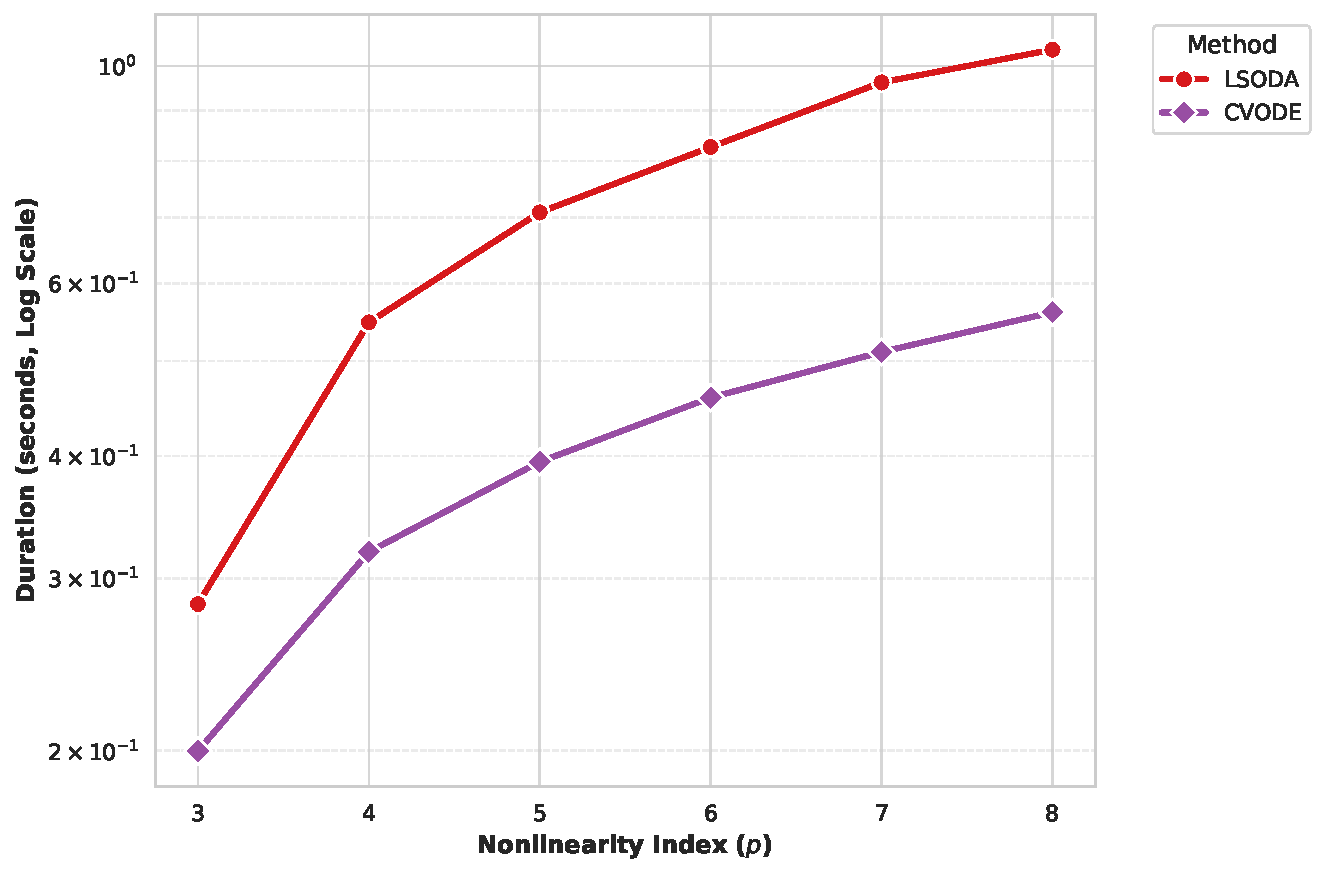
\includegraphics[width=\textwidth]{images/extreme_p_scaling.pdf}
  \caption{Execution time scaling for LSODA and CVODE as the nonlinearity index \(p\) is pushed into the strongly degenerate regime (\(p = 3.0\) to \(8.0\)).}
  \label{fig:extreme-p}
\end{figure}
